\documentclass{acmsiggraph}                     % final
%\documentclass[annualconference]{acmsiggraph}  % final (annual conference)
%\documentclass[review]{acmsiggraph}            % review
%\documentclass[widereview]{acmsiggraph}        % wide-spaced review
%\documentclass[preprint]{acmsiggraph}          % preprint

%% Uncomment one of the five lines above depending on where your paper is
%% in the conference process. ``review'' and ``widereview'' are for review
%% submission, ``preprint'' is for pre-publication, and ``final'' is for
%% the version to be printed. The ``final'' variant will accept the 
%% ``annualconference'' parameter, which changes the height of the space
%% left clear for the ACM copyright information.

%% The 'helvet' and 'times' packages define the typefaces used for
%% serif and sans serif type in this document. Computer Modern Roman 
%% is used for mathematics typesetting. The scale factor is set to .92
%% to bring the sans-serif type in line with the serif type.

\usepackage[scaled=.92]{helvet}
\usepackage{times}
\usepackage{latexsym}
\usepackage{url}

%% The 'graphicx' package allows for the inclusion of EPS figures.

\usepackage{graphicx}

%% use this for zero \parindent and non-zero \parskip, intelligently.

\usepackage{parskip}

%% Optional: the 'caption' package provides a nicer-looking replacement
%% for the standard caption environment. With 'labelfont=bf,'textfont=it',
%% caption labels are bold and caption text is italic.

\usepackage[labelfont=bf,textfont=it]{caption}

%% If you are submitting a paper to the annual conference, please replace 
%% the value ``0'' below with the numeric value of your OnlineID. 
%% If you are not submitting this paper to the annual conference, 
%% you may safely leave it at ``0'' -- it will not be included in the output.

\usepackage{listings}
\usepackage{alltt}
\usepackage{subfigure}

%%\usepackage[caption=false]{subfig}

%%\onlineid{paper1041}

%% Paper title.

\title{The X3D Geospatial Component: X3DOM implementation of GeoOrigin, GeoLocation, GeoViewpoint, and GeoPositionInterpolator nodes}

%% Author and Affiliation (single author).

%%\author{Roy G. Biv\thanks{e-mail: roy.g.biv@aol.com}\\Allied Widgets Research}

%% Author and Affiliation (multiple authors).


\author{Andreas Plesch\thanks{e-mail: andreasplesch@gmail.com}\\Harvard University
\and Michael McCann\thanks{e-mail: mccann@mbari.org}\\MBARI
\and Don Brutzman\thanks{e-mail: brutzman@nps.edu}\\Naval Postgraduate School}


%% Keywords that describe your work.

\keywords{3-D Geography, X3D, geospatial, X3D-Geospatial, X3D-Earth, X3DOM }

%%%%%% START OF THE PAPER %%%%%%

\begin{document}

%%\teaser{
%%\subfigure{
%%\includegraphics[width=7in]{STOQSUIscreencapture.png}
%%
%%}

%%\caption{Screen capture of the STOQS web application showing underwater sensor data off the coast of southern California.}
%%\label{fig:STOQSscreencapture}
%%}




%% The ``\maketitle'' command must be the first command after the
%% ``\begin{document}'' command. It prepares and prints the title block.

\maketitle

%% Abstract section.

\begin{abstract}

We present new implementations of important X3D nodes which enable a large class of geospatial applications in standard web browsers. We have chosen the freely available X3DOM code base as an implementation framework since it provides a very functional set of X3D nodes along with a broad selection of support functionality. In our implementations of the GeoOrigin, GeoLocation, GeoViewpoint and GeoPositionInterpolator nodes, we fully conform to the ISO specification and use well known example scenes as references for correctness. While GeoOrigin is deprecated in the v3.3 of the specification, we demonstrate that limited precision in the webgl rendering pipeline still make its use desirable at least until alternative solutions are formalized and coded. GeoLocation and GeoViewpoint nodes require specific alignments of coordinate systems which we document in detail. In addition, GeoViewpoint has the property to control navigation speed which conceptually conflicts with user speed control. We resolve this conflict by using relative speed and also make this control optional. Somewhat terse language in the GeoPositionInterpolator specification required clarification of its existing usage and inspired an option for coordinate interpolation along great circles which is often the expected interpolation path in global scenes. Finally, all functionality was integrated into current, stable releases of the X3DOM distribution available from www.x3dom.org.

\end{abstract}

%% ACM Computing Review (CR) categories. 
%% See <http://www.acm.org/class/1998/> for details.
%% The ``\CRcat'' command takes four arguments.

\begin{CRcatlist}
\CRcat{I.3.7}{Computing Methodologies}{Computer Graphics}{Three-Dimensional Graphics and Realism}
\end{CRcatlist}

%% The ``\keywordlist'' command prints out the keywords.
\keywordlist

\section{Background}

\copyrightspace
%% The ``\copyrightspace'' command must be the first command after the 
%% start of the first section of the body of your paper. It ensures the
%% copyright space is left at the bottom of the first column on the first
%% page of your paper.

The ability to use geospatially well registered geometry and geospatially informed data structures was recognized as an important concept early in the development of virtual worlds where they were to reflect the physical word. Consequently, specialized geospatial nodes found their way into the definition of the Virtual Reality Modeling Language (VRML) in the late 1990s \cite{reddy2000}. In the early 2010s, the successor to VRML --- X3D --- gained traction and became significantly more accessible by the availability of X3DOM, an openly developed JavaScript X3D interpreter and renderer \cite{behr09}, while webgl became a standard feature in web browsers. X3D is designed to be modular \cite{x3d05} and retains geospatial functionality in a dedicated geospatial component. Here, we present new implementations of important nodes of the geospatial component within the X3DOM code framework.


\section{Motivation}

The X3D geospatial component occupies a unique space between the worlds of Geographical Information System (GIS) and 3D computer graphics. GIS traditionally works with a map based representation of geographical features while treating the third dimension of elevation or depth as attribute or property rather than an independent dimension equally relevant to the map dimensions. Although modern GIS systems (PostGIS or ArcGIS, for example) allow use of three dimensional coordinates in specifying geometrical elements, they remain based on a 2D, map based world view both in terms of analysis and visualization. On the other hand, there are many inherently three dimensional geospatial data sets and problems which makes them more difficult to use or solve in a GIS environment.  Examples include geological and geophysical data of the subsurface, atmospheric and climate data, or oceanographic data concerned with part or the full volume of what occupies the majority of the planet. In fact, global data sets benefit strongly from a 3D analysis and visualization environment since the shape of the Geoid is not suited to faithful projection onto a 2D plane. The X3D geospatial components addresses this need in terms of visualization. At the same time it is part of the full X3D scene graph which provides the basis for interactive modes of exploration of geospatial data sets which are generally not targeted by GIS. At a practical level, essentially unlimited sharing of visualizations of geospatial 3D data sets becomes straightforward with the use of the X3DOM geospatial component and world wide web technologies.


\section{The X3D geospatial component and digital globes}

Digital globes, either web based such as Cesium \cite{cesium15} or standalone such as Google Earth \cite{googleearth15}, may be seen to offer similar functionality as the X3D geospatial component. After all, they also portray the physical Earth in 3D. However, it is important to state that the X3D geospatial component targets generalized functionality and is not restricted to the planet's surface. In fact, given sufficient data sets, a digital globe could be declared in an X3D scene, and, given sufficient performance, then rendered in a geospatially enabled X3D browser. In this context a digital globe can be seen as just one of many possible applications of X3D and its geospatial component. The newly implemented nodes then could work towards enhancing such an X3D-declared, digital globe with user content such as buildings, mines or dynamic submarines, user views, or user interactions.

\section{The Nodes}

\subsection{The geocentric coordinate system}

Before we present details on functionality and implementation of the newly available nodes, it is useful to outline the use of coordinate systems in the X3D geospatial component. While in regular X3D scenes the XZ plane is considered horizontal and the +Y direction as pointing vertically upwards, in geospatial scenes the X,Y and Z coordinates are used as geocentric coordinates. The origin of the geocentric coordinate system is the center of the planet, the +X direction points to 0 degrees longitude, the +Z direction points to the north pole, and the +Y direction point to 90 degrees longitude east. The units are meters. Using this definition allows use of any X3D node with the proper geocentric coordinates in conjunction with geospatial nodes. This may be considered useful in praxis where an external geospatial database provides data and also the necessary coordinate transformations.

\subsection{GeoOrigin}

The GeoOrigin node is a helper node, which is deprecated but still useful for improving rendering precision due to limitations of the webGL rendering pipeline. While JavaScript uses double precision floating point numbers for any numeric operation, webGL seems to only use single precision floating point numbers. This limits precision for geocentric coordinates which are on the order of 106 meters to about 1 meter which is not sufficient for many applications (Fig.~\ref{fig:GeoOriginDiagram}). The GeoOrigin node works by providing a local origin the coordinates of which are then subtracted from node coordinates to arrive at smaller numbers to pass on to the rendering pipeline for greater precision (Fig.~\ref{fig:GeoOriginImage}).

\begin{figure}[htbp]
\centering
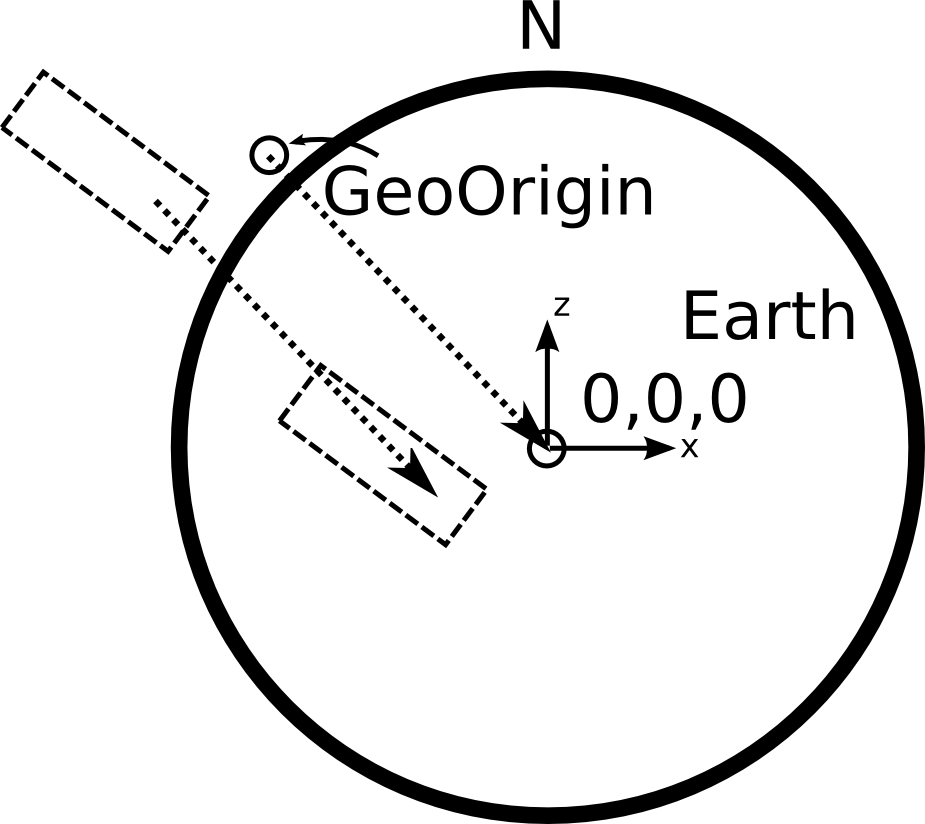
\includegraphics[width=2.0in]{GeoOriginDiagram.png}
\caption{The position of a GeoOrigin node is given in the vicinity of a geospatial scene (stippled box). The scene is translated towards the X3D coordinate origin for greater coordinate precision.}
\label{fig:GeoOriginDiagram}
\end{figure}


A peculiar feature of the GeoOrigin node is that although only a single definition of it is sensible in a geospatial scene, it needs to be provided for each node separately as a child node.

\begin{figure*}[htbp]
\centering
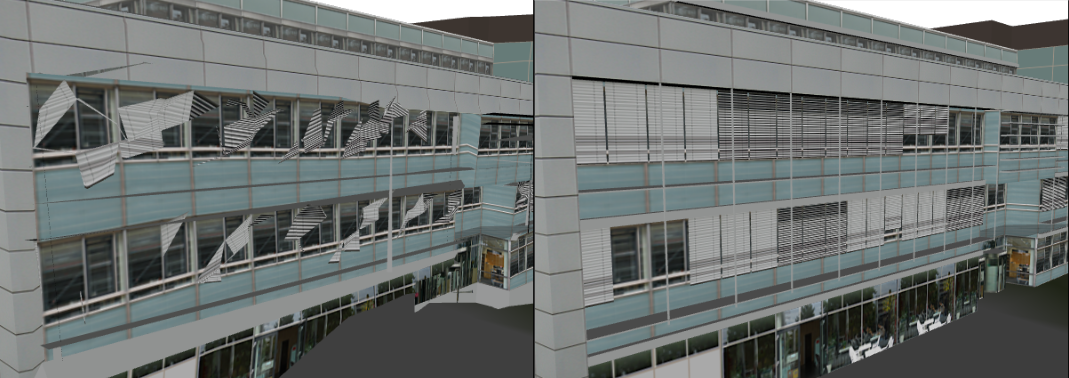
\includegraphics[width=6.6in]{GeoOriginImage.png}
\caption{An architectural X3D scene (x3dom.org) without (left) and with (right) use of a GeoOrigin node. Without GeoOrigin lack of precision leads to rendering artefacts.}
\label{fig:GeoOriginImage}
\end{figure*}

Another feature of the GeoOrgin node is the rotateYUp field. It is a somewhat difficult concept to grasp. It rotates the local (geospatial) Up (skywards) direction to the scene +Y direction. In that sense it may be thought of as "rotateUptoY". In the ISO specification language this rotation is called an alignment which leaves the point about which the rotation is performed undefined. Similarly, the specification is silent on the axis about which the rotation may be performed. In our implementation we choose the GeoOrigin point as the point of rotation (Fig.~\ref{fig:RotateYUp}) and the axis of rotation such that the direction pointing north becomes aligned with the scene -Z direction. The local (geospatial) Up (skywards) direction is also not strictly defined in the specification. It can differ slightly from vertex to vertex in a geospatial scene or even significantly in the case of large, country  or continent sized scenes. In our implementation we choose to use the Up direction at the position of the GeoOrigin point which is constant throughout a scene (Fig.~\ref{fig:RotateYUp}).

\begin{figure}[htbp]
\centering
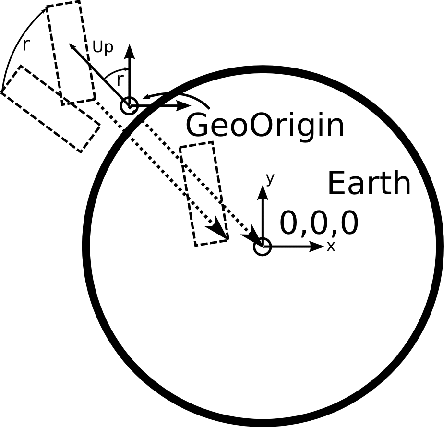
\includegraphics[width=2.0in]{RotateYUp.png}
\caption{This slice of the earth through the equator shows how the RotateYUp rotation of the GeoOrigin field works in our implementation. The local Up direction is given at the position of the GeoOrigin which is then aligned with the Y axis. The rotation occurs about the position of the GeoOrigin point.}
\label{fig:RotateYUp}
\end{figure}

Therefore, for nodes which have a GeoOrigin node defined, our code implements this sequence of transformation: First the GeoOrigin coordinates are subtracted. Then, if rotateYUp is requested, a rotation matrix is computed based on how a GeoLocation (see below) node would transform geometry with the GeoOrigin position as the GeoLocation position. Finally, the calculated rotation matrix is inverted and applied to each vertex of the node.

Alternatives to solving the precision issue exist \cite{mccann09} (McCann et al., 2009) but still need refinement and implementation.


\subsection{GeoLocation}

The GeoLocation node is in effect a specialized Transform node to translate the geospatially unregistered child node's origin to the provided geospatial coordinates, and to rotate the child's +Y direction to the local Up direction (perpendicular to geoid) as well as the child's -Z direction towards the local north direction (along the longitude) (Fig.~\ref{fig:GeoLocationDiagram}). It needs the (inverse) projection from geocentric to latitude and longitude coordinates of the provided geospatial position.

\begin{figure}[htbp]
\centering
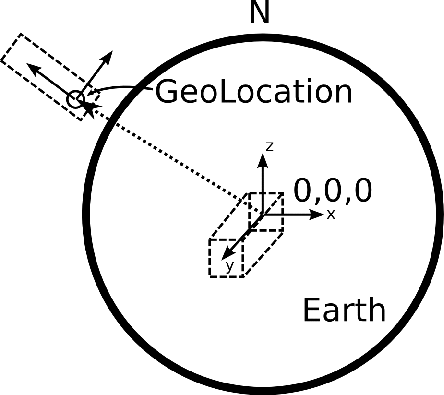
\includegraphics[width=2.0in]{GeoLocationDiagram.png}
\caption{This slice of earth through the longitudinal plane at the position of a GeoLocation node shows how a child node (stippled box) is rotated to align the Y axis with the Up direction and translated to the position of the GeoLocation.}
\label{fig:GeoLocationDiagram}
\end{figure}

We implement this transformation by first calculating the quaternion representations qX and qZ  of two rotations: about the X axis by 180 - latitude degrees to align +Y with local Up and about the Z axis by 90 + longitude degrees to align -Z with longitude towards north. The product qZ * qX of these quaternions is converted to a rotation matrix rM. Then a transformation matrix tM is constructed for a translation to the GeoLocation position. The final transformation matrix is calculated as the product of the rotation and translation matrices tM * rM.

A conceptual complication occurs when rotateYUp is requested in a GeoOrigin node in conjunction with the GeoLocation node. This will rotate the Up direction back to +Y but note that the rotation occurs not about the same point: the GeoLocation position is likely different from the position of the provided GeoOrigin (compare Fig.~\ref{fig:RotateYUp} and Fig.~\ref{fig:GeoLocationDiagram}). Therefore, an implementation cannot just skip both rotations. Instead, the full transformation path has to be traversed (by matrix multiplication): Geolocation rotation (about child origin), Geolocation translation, GeoOrigin (back) translation, rotateYUp rotation.

\begin{figure}[htbp]
\centering
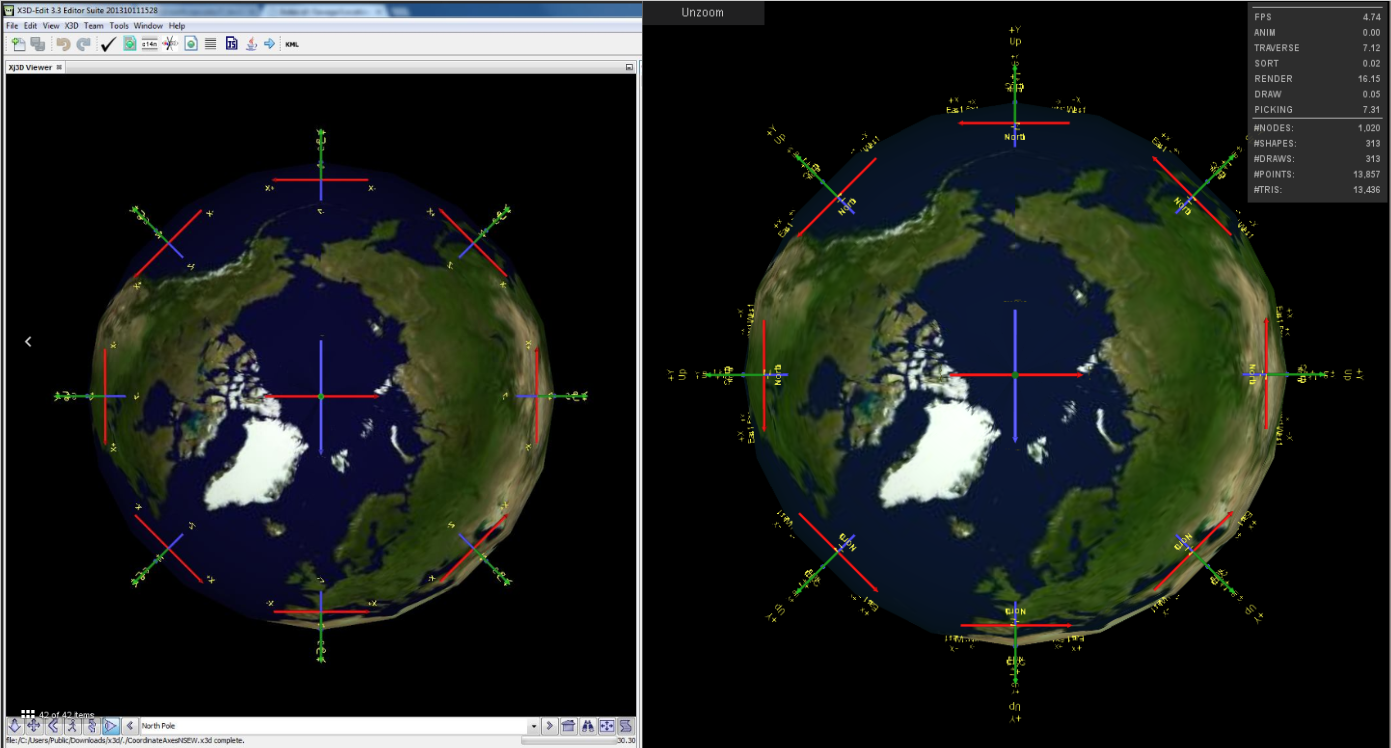
\includegraphics[width=3.3in]{Axes_NSEW.png}
\caption{The left side shows the 'Geospatial Coordinate Axes Nsew Example' slightly modified from the Web3D X3D example archive as rendered by the xj3d browser, and the same example scene as rendered by X3DOM. The colored vectors are based on a single coordinate axes scene and then properly positioned at various locations by GeoLocation nodes.}
\label{fig:Axes_NSEW.png}
\end{figure}

\subsection{GeoViewpoint}

The GeoViewpoint is a specialized Viewpoint node with the ability to provide its position in geospatial coordinates and its view orientation with respect to the local Up direction. It also has an option to adjust navigation speed based on elevation.

Consequently our implementation is based on the X3DOM Viewpoint code. All fields defined in the ISO specification are supported, including the deprecated headlight and navType fields. These two fields are by default "undefined" to allow for the equivalent NavigationInfo node fields to take effect. If used, they take precedence over the currently bound NavigationInfo node fields.

In the X3DOM framework a Viewpoint node is expected to deliver a view matrix on request. Our code first computes a viewpoint rotation matrix vrM as the product rM * oM of a rotation matrix rM and the node provided orientation oM converted to matrix where rM is computed as in a GeoLocation node including the adjustments for rotateYUp using the position of the Geoviewpoint. Finally, the view matrix is derived as the inverse of the product tM * vrM of the translation matrix constructed from the Geoviewpoint position tM and the viewpoint rotation matrix vrM.

One additional field of type SFBool called elevationScaling is introduced. It controls the use of navigation speed scaling by avatar elevation above ground level and is turned on (true) by default as the ISO specification suggests. The specification's suggestion to compute the scaling factor as elevation in meters divided by 10 is adopted. Elevation scaled speed is not used for examine and examine like navigation modes. Even when elevation scaling of speed is turned on users still can modify their speeds by a user speed factor, eg. with the +/- keys. This is accomplished by treating elevation scaled speed not as absolute speed but as a factor to the user defined speed. 

The ISO specification does not elaborate on if or how elevation scaling should be updated during navigation. For many purposes it may suffice to base initial navigation speed on the elevation of the Geoviewpoint and ignore changes of avatar elevation during navigation. In our X3DOM implementation, however, the speed is updated frequently which allows for seamless exploration from great height at satellite elevation down to the height of a person walking. As the implementation of elevation scaling dynamically updates speed, it relies on getViewMatrix() being called from Viewarea.js during navigation.

An interesting side effect of speed scaling by elevation is that as the avatar approaches ground level with an elevation of zero the scaling factor also approaches zero. Therefore the avatar would stop moving at ground level and would be trapped. Therefore we restrict  the scaling factor to not fall below 1 at any elevation.

Although the ISO specification language references elevation as measured from the topographic ground surface, we use elevation measured from the geoid (approximated by ellipsoids) surface for efficiency.

We also discussed the situation when the avatar is below ground level or sea level, eg. when elevation is negative. Currently, we simply use the absolute magnitude of elevation. Another useful option would be the ability to provide a local datum elevation as reference height from which elevation could be measured.

Other details include resetting the center of rotation when the viewpoint is reset, and support of the rotateYUp field if a GeoOrigin child node is used. RotateYUp allows navigation modes which assume that the Up direction aligns with the positive Y axis to work correctly.


\subsection{GeoPositionInterpolator}

The GeoPositionInterpolator node works similar to the PositionInterpolator node. It interpolates between geospatial coordinates and outputs both coordinates in the specified reference system (geoSystem) and also scene coordinates. The ISO specification is very clear that the geovalue\_changed field contains the interpolated geo-coordinates. The specification wording for value\_changed, however, is somewhat ambiguous. The initial implementation of the node \cite{reddy2000} and feedback from long-time users strongly suggest that the value\_changed field provides scene coordinates. Scene coordinates are geocentric coordinates adjusted for a GeoOrigin when provided.

The specification is silent on what kind of interpolation is provided by the node. Early \cite{reddy2000} and most existing implementations (xj3d, freewrl) of the node use linear interpolation of the coordinates, before their transformation to geocentric coordinates. On a planar surface or for small distances on the geoid, this makes sense and is what would be expected. Going to large distances on the geoid, for example when looking at an intercontinental flight path or at satellite tracks, interpolation along the great circle arc between two points becomes more desirable. A great circle measures the shortest distance between two points on a sphere and is what is often shown for plane and satellite tracks. Therefore the X3DOM implementation of the node introduces an additional field called onGreatCircle. It lets a user choose between linear and great circle type interpolation. Although at small distances a  straight line is closely approximated by a great circle, the onGreatCircle field is set to false by default for performance and compatibility reasons. This means by default the node will use linear interpolation to interpolate between coordinates. The elevation coordinate is linearly interpolated in both interpolation modes.

\begin{figure}[htbp]
\centering
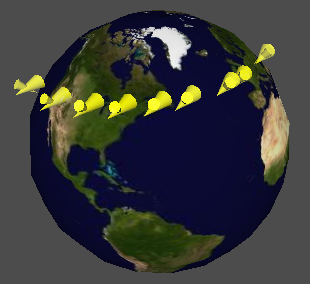
\includegraphics[width=3.3in]{GeoPositionInterpolator1.png}
\caption{A GeoPositionInterpolator node interpolates the latitude and longitude coordinates of a double cone linearly between London and San Francisco. The scene is adopted from the A2 Animated Geoviewpoint example scene at the web3d archive.}
\label{fig:GeoPositionInterpolator1.png}
\end{figure}

\begin{figure}[htbp]
\centering
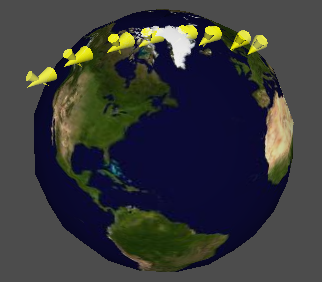
\includegraphics[width=3.3in]{GeoPositionInterpolator2.png}
\caption{A GeoPositionInterpolator node interpolates the position of a double cone on a great circle between London and San Francisco.}
\label{fig:GeoPositionInterpolator2.png}
\end{figure}

In detail, the code first transforms all key values to geocentric coordinates to a new array when the node is encountered or was changed.  For great circle interpolation, the code then interpolates the geocentric coordinates for the requested key using this new array via a slerp algorithm (Shoemake, 1985) which has the property of constant speed, eg. linearly interpolates the arc angle between two key positions. The geovalue\_changed output is derived from the interpolated geocentric coordinates by inverse projection depending on the geoSystem. Finally, the  value\_changed output is computed from the interpolated geocentric coordinates by taking into account a GeoOrigin if provided. Altogether, these steps involve one coordinate projection per point and 1 or 2 matrix multiplications: geoOrigin translation and rotateYUp rotation.

For linear interpolation, the code interpolates the geovalue\_changed output using the original key value array. Then, geocentric coordinates are derived from the interpolated geospatial coordinates depending on the geoSystem. Finally, the  value\_changed output is computed from the interpolated geocentric coordinates by taking into account a GeoOrigin if provided. Altogether, these steps involve one coordinate projection per point and 1 or 2 matrix multiplications: geoOrigin translation and rotateYUp rotation.

In terms of performance, the great circle interpolation suffers a bit from having to perform a slerp calculation. However, slerp is very efficient. In fact, limited profiling indicates that the ROUTE mechanism used with a the GeoInterpolator node may take up more time than the interpolation itself independent of its type.



\section{Applications}

The availability of the geospatial component in a web browser via X3DOM allows for development of rich  web apps but also for very targeted application which rely exclusively on the X3D scene graph and standard X3DOM navigation functionality. We briefly describe examples for each scenario.

The Monterey Bay Aquarium Research Institute designed the Spatial Temporal Oceanographic Query System (STOQS) \cite{mccann14} to create new capabilities for scientists to gain insight from their data. STOQS employs open standards and is a 100% free and open source project. It includes a web-based graphical user interface where X3D Geospatial has been integrated to enable 3D geospatial data visualization. The system uses most of the presented geospatial nodes and is actively developed.

\begin{figure}[htbp]
\centering
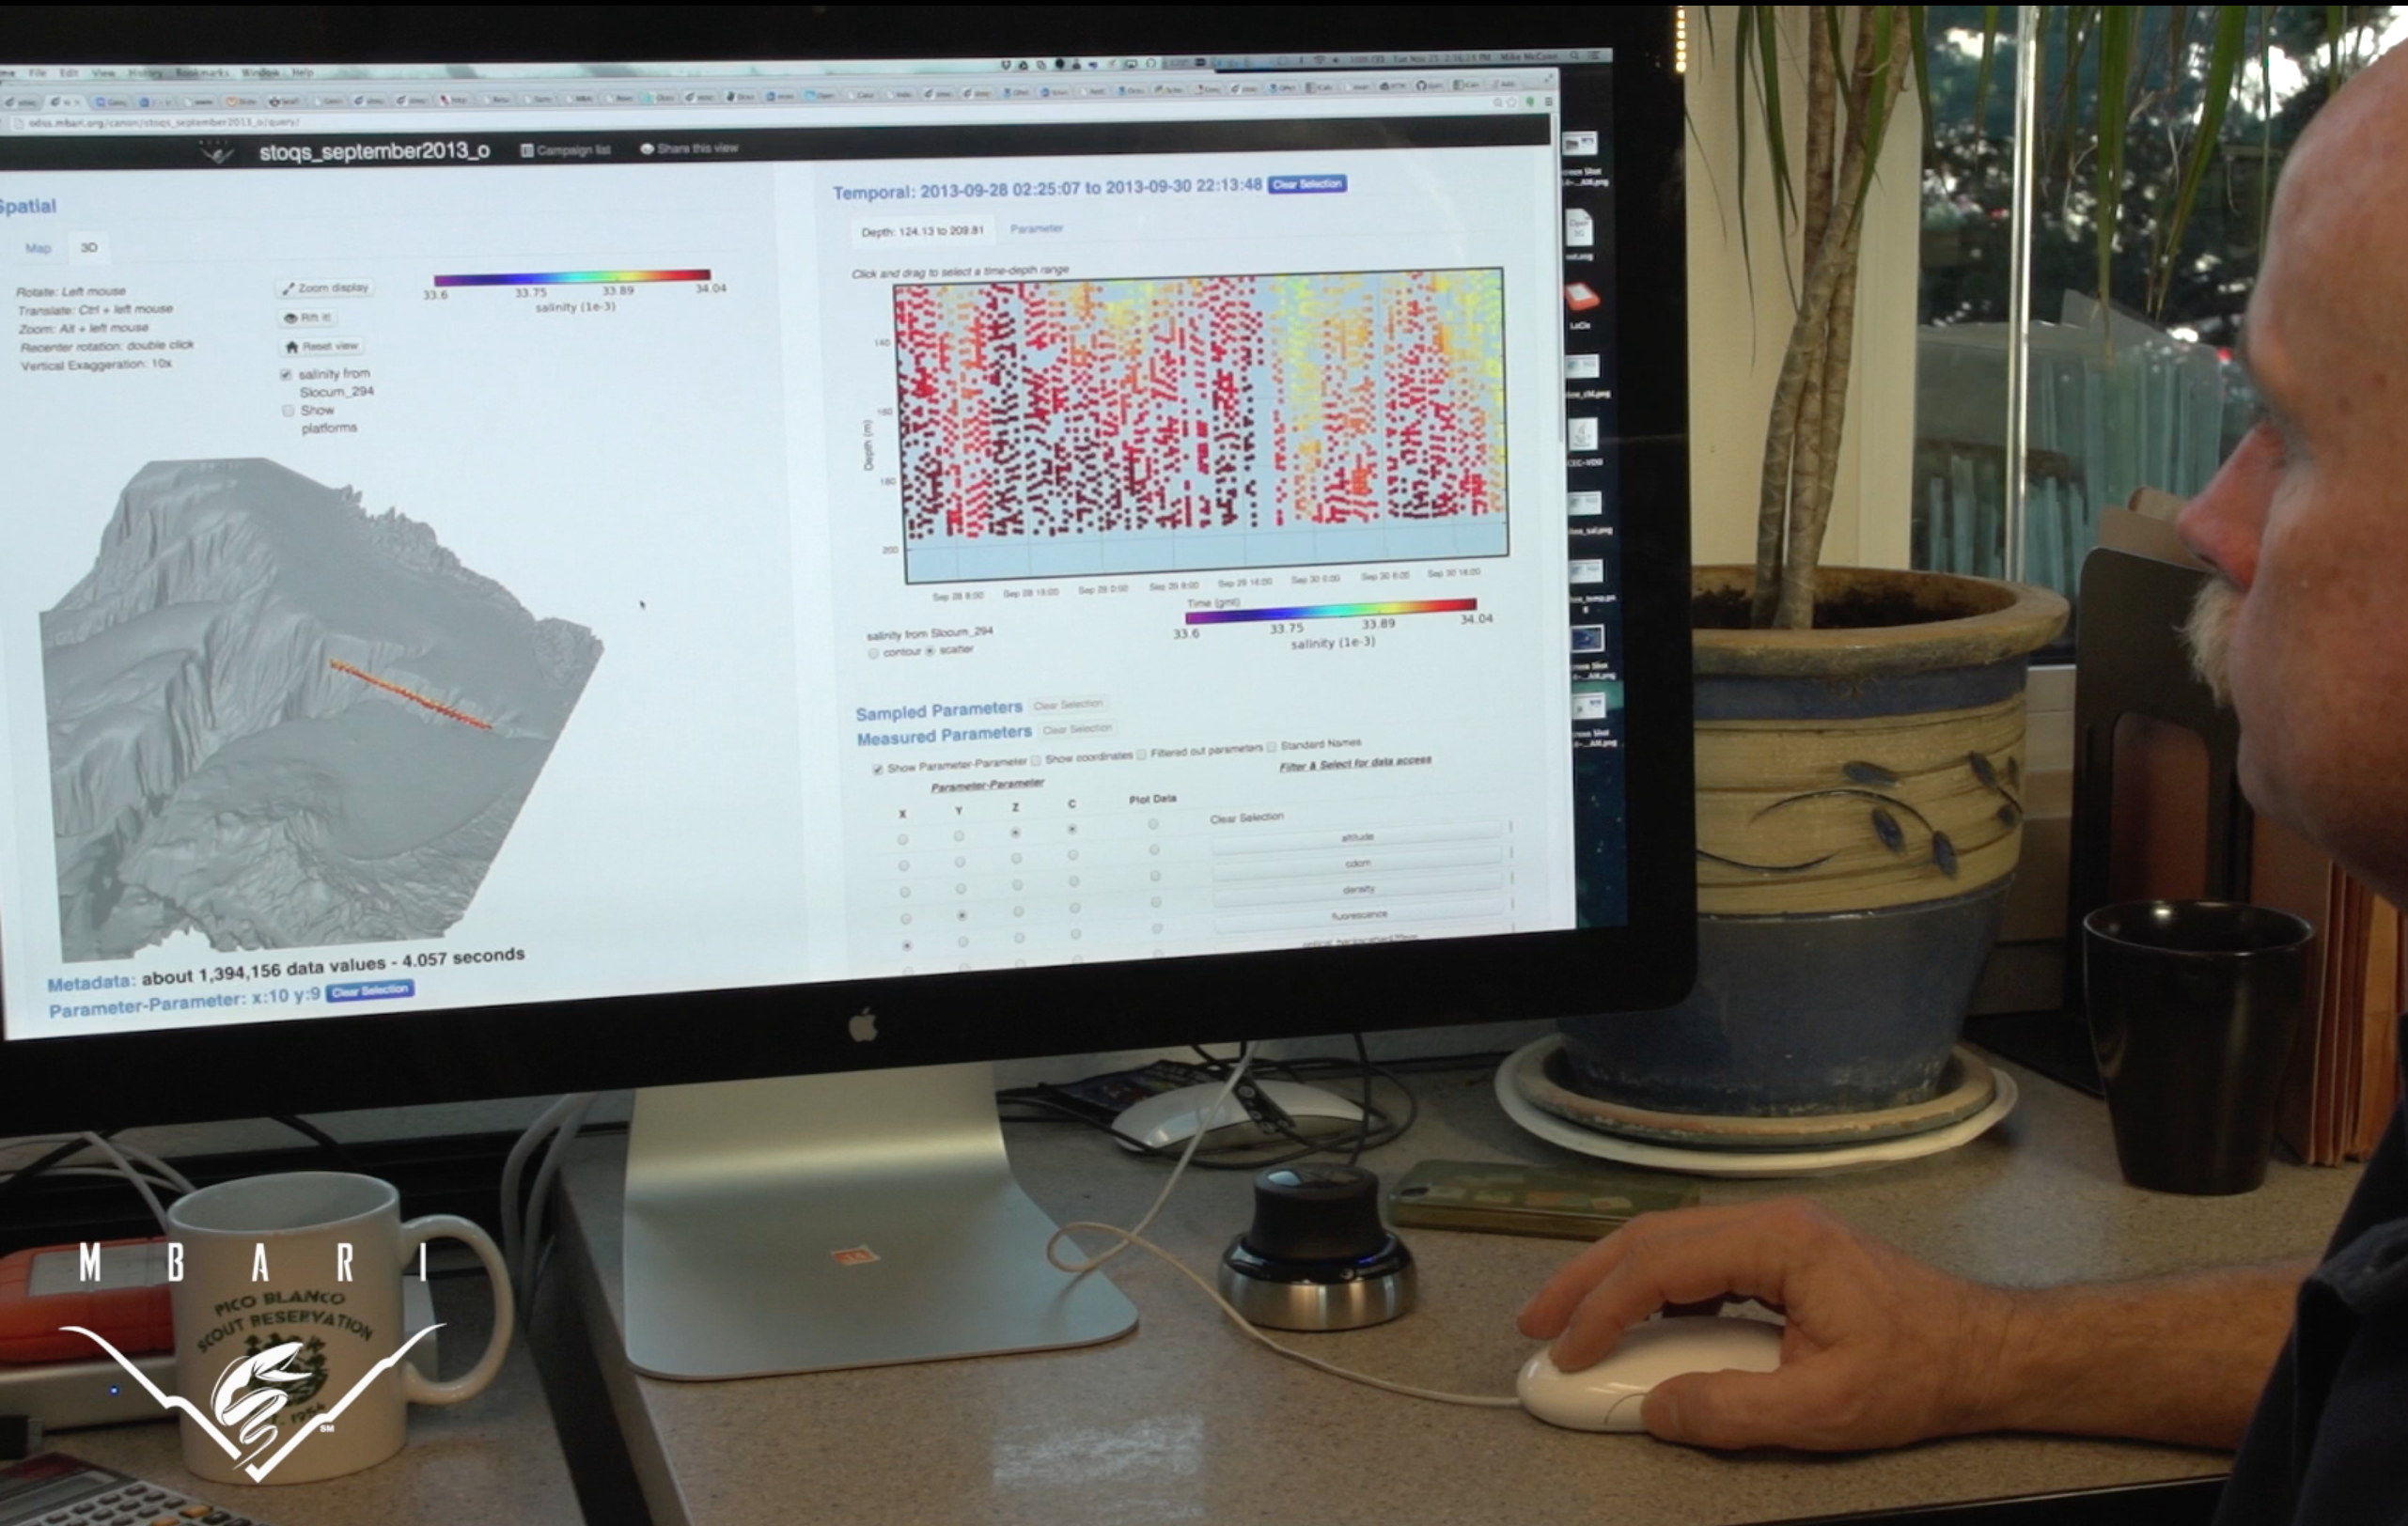
\includegraphics[width=3.3in]{Application_STOQS.png}
\caption{The X3D geospatial component makes complex oceanographic data easy to visualize and understand. This is frame from a video about the STOQS project that may be viewed on YouTube.}
\label{fig:Application_STOQS.png}
\end{figure}

A simple use case is the easily deployable and accessible visualization of the Community Fault Model for Southern California (Plesch et al., 2007) which is a foundational data set for earthquake science and used by diverse set of geoscientists. Using the X3DOM geospatial component it was possible to make available multiple versions of the data set using limited resources under dead line pressure (SGER, 2014).

\begin{figure}[htbp]
\centering
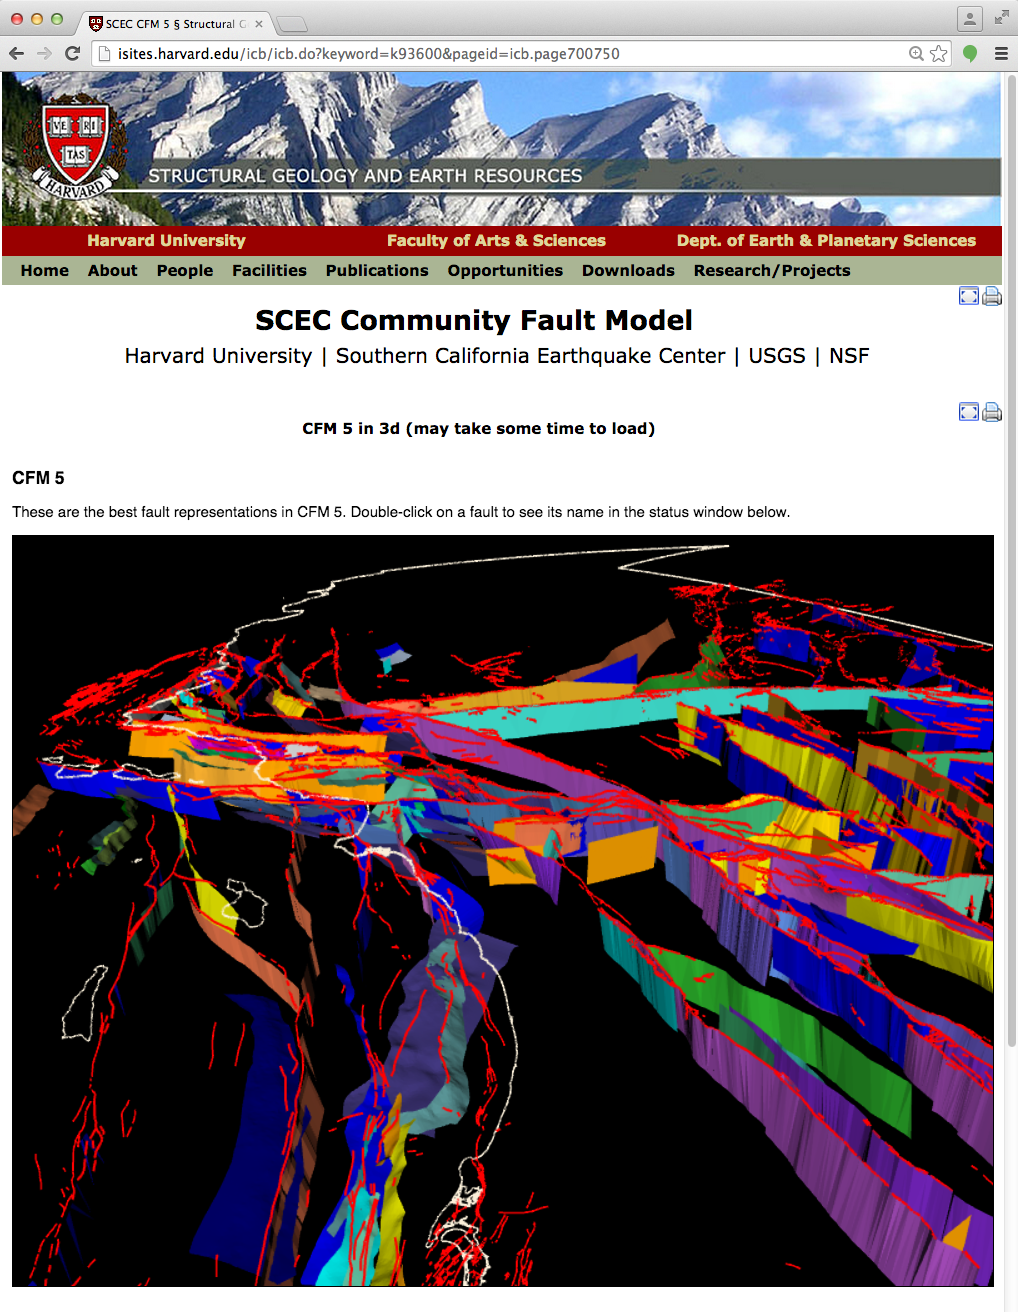
\includegraphics[width=3.3in]{Application_SCEC.png}
\caption{The X3D geospatial component makes it possible for a wide audience to explore a 3D geological model of earthquake faults in California by just opening a web page.}
\label{fig:Application_SCEC.png}
\end{figure}


\section{Summary}

We present new implementations of important X3D nodes which enable a large class of geospatial applications in standard web browsers. In our implementations of the GeoOrigin, GeoLocation, GeoViewpoint and GeoPositionInterpolator nodes, we fully conform to the ISO specification and use example scenes from well known sources as references for correctness. We demonstrate that limited precision in the webgl rendering pipeline still make the availability of a GeoOrigin desirable at least until alternative solutions are formalized and coded. GeoLocation and GeoViewpoint nodes require specific alignments of coordinate systems which we document in detail including the treatment of the rotateYUp field. In addition, GeoViewpoint has the property to control navigation speed which conceptually conflicts with user speed control. We resolve this conflict by using relative speed and also make this control optional. Somewhat terse language in the GeoPositionInterpolator specification required clarification of its existing usage and inspired an option for coordinate interpolation along great circles which is often the expected interpolation path in global scenes. Finally, all functionality was integrated into current, stable releases of the X3DOM distribution available from www.x3dom.org.







\bibliographystyle{acmsiggraph}
\nocite{*}
\bibliography{X3DGeospatialComponent}




\end{document}
